% Arquivo LaTeX de exemplo de dissertação/tese a ser apresentada à CPG do IME-USP
%
% Criação: Jesús P. Mena-Chalco
% Revisão: Fabio Kon e Paulo Feofiloff
% Adaptação para UTF8, biblatex e outras melhorias: Nelson Lago
%
% Except where otherwise indicated, these files are distributed under
% the MIT Licence. The example text, which includes the tutorial and
% examples as well as the explanatory comments in the source, are
% available under the Creative Commons Attribution International
% Licence, v4.0 (CC-BY 4.0) - https://creativecommons.org/licenses/by/4.0/


\documentclass[a4paper,12pt,twoside,brazilian,english]{book}
\usepackage{style/imegoodies}
\usepackage[thesis]{style/imelooks}
\graphicspath{{figuras/},{fig/},{logos/},{img/},{images/},{imagens/}}

% Comandos rápidos para mudar de língua:
% \en -> muda para o inglês
% \br -> muda para o português
\babeltags{br = brazilian, en = english}

%%%%%%%%%%%%%%%%%%%%%%%%%%%%%%%%%%%%%%%%%%%%%%%%%%%%%%%%%%%%%%%%%%%%%%%%%%%%%%%%
%%%%%%%%%%%%%%%%%%%%%%%%%%%%%%%%%% METADADOS %%%%%%%%%%%%%%%%%%%%%%%%%%%%%%%%%%%
%%%%%%%%%%%%%%%%%%%%%%%%%%%%%%%%%%%%%%%%%%%%%%%%%%%%%%%%%%%%%%%%%%%%%%%%%%%%%%%%

\addbibresource{bibliografia.bib}

\babelhyphenation{documentclass latexmk soft-ware clsguide}
\babelhyphenation[brazilian]{Fu-la-no}
\babelhyphenation[english]{what-ever}

\title{An implementation of the Rainbow Version of Dirac's Theorem}[]

\author[fem]{Nathan Luiz, Willian Mori}

\def\profa{Prof\kern.02em.\kern-.07emª\kern.07em}
\def\dra{Dr\kern-.04em.\kern-.11emª\kern.07em}

\orientador[fem]{Yoshiko Wakabayashi} % TODO: titulo 

\tipotese{
  tcc,
  programa={Computer Science},
}
\defesa{
  local={São Paulo},
  data=1999-11-11, % YYYY-MM-DD
}
\direitos{CC-BY}
\fichacatalografica{}

%%%%%%%%%%%%%%%%%%%%%%%%%%%%%%%%%%%%%%%%%%%%%%%%%%%%%%%%%%%%%%%%%%%%%%%%%%%%%%%%
%%%%%%%%%%%%%%%%%%%%%%% AQUI COMEÇA O CONTEÚDO DE FATO %%%%%%%%%%%%%%%%%%%%%%%%%
%%%%%%%%%%%%%%%%%%%%%%%%%%%%%%%%%%%%%%%%%%%%%%%%%%%%%%%%%%%%%%%%%%%%%%%%%%%%%%%%

\begin{document}

%%%%%%%%%%%%%%%%%%%%%%%%%%% CAPA E PÁGINAS INICIAIS %%%%%%%%%%%%%%%%%%%%%%%%%%%%

\frontmatter
\pagestyle{plain}
\onehalfspacing
\maketitle

%%%%%%%%%%%%%%%% DEDICATÓRIA, AGRADECIMENTOS, RESUMO/ABSTRACT %%%%%%%%%%%%%%%%%%

\pagenumbering{roman}

\chapter*{Acknowledgment}
% TODO

%%%%%%%%%%%%%%%%%%%%%%%%%%% LISTAS DE FIGURAS ETC. %%%%%%%%%%%%%%%%%%%%%%%%%%%%%

\tableofcontents

%%%%%%%%%%%%%%%%%%%%%%%%%%%%%%%% CAPÍTULOS %%%%%%%%%%%%%%%%%%%%%%%%%%%%%%%%%%%%%

\mainmatter
\singlespacing

\pagestyle{mainmatter}
%!TeX root=../tese.tex
%("dica" para o editor de texto: este arquivo é parte de um documento maior)
% para saber mais: https://tex.stackexchange.com/q/78101

\chapter{Introduction}

O problema estudado neste artigo é relativamente recente, embora suas origens remontem a conceitos clássicos. 
Em 1978, Caccetta e Häggkvist formularam a conjectura de que todo dígrafo de ordem $n$ com grau 
mínimo $d$ possui um circuito direcionado de tamanho no máximo $\lceil n/d \rceil$. Essa 
conjectura marcou o início de investigações sobre circuitos em grafos com restrições de grau.

Quase quatro décadas depois, em 2017, Ron Aharoni, do Departamento de Matemática do Technion, 
propôs uma versão mais forte dessa conjectura utilizando a versão Rainbow. Sua conjectura
afirma que, dado um grafo $G$ de ordem $n$ com arestas coloridas em $n$ cores, onde cada cor 
aparece em no máximo $r$ arestas, existe um circuito rainbow de tamanho no máximo $\lceil n/r \rceil$.

Em 2019, Felix Joos, professor na Universidade de Heidelberg, e Jaehoon Kim, professor associado 
no KAIST, conseguiram provar a existência de um circuito hamiltoniano rainbow em uma coleção de 
grafos definidos sobre o mesmo conjunto de vértices, com arestas coloridas de forma distinta, 
que satisfazem a condição de Dirac. Essa prova deu um forte suporte à conjectura de Aharoni.

O trabalho de Joos e Kim utilizou técnicas simples e elegantes, mas não triviais, 
que permitiram o desenvolvimento de um algoritmo cúbico no número de vértices. Além disso, eles 
estenderam seus resultados para a existência de um matching perfeito rainbow.

Mais recentemente, em 2023, Liqing Gao e Jian Wang, pesquisadores chineses, publicaram um artigo 
que estende o problema ao provar a existência de um circuito hamiltoniano rainbow em grafos que 
satisfazem a condição de Ore, utilizando a ferramenta do "shifting operator". Esta técnica, 
desenvolvida por Erdös, Ko e Rado, é amplamente utilizada na teoria dos conjuntos extremais e 
permitiu um avanço significativo na resolução deste problema. Porém, não iremos abordar este
trabalho em detalhes neste artigo.

Este trabalho está estruturado da seguinte forma: no Capítulo 2, explicaremos e provaremos a 
condição de Dirac. No Capítulo 3, abordaremos a versão Rainbow dos algoritmos, essencial para a 
compreensão do algoritmo final. No Capítulo 4, implementaremos o algoritmo baseado no trabalho 
de Joos e Kim, apresentando pseudocódigos e provando a corretude do algoritmo. No Capítulo 5, 
incluiremos uma animação gráfica para ilustrar o funcionamento do algoritmo. Finalmente, no 
Capítulo 6, faremos as considerações finais sobre o trabalho desenvolvido.

Todo o código-fonte utilizado neste projeto está disponível em $nosso-repo$ 
O código foi escrito em C++, utilizando a biblioteca Boost, e em Python, no qual tem suporte para 
uma animação que foi feita usando o framework Graph-Tool.


\pagestyle{mainmatter}
%!TeX root=../tese.tex
%("dica" para o editor de texto: este arquivo é parte de um documento maior)
% para saber mais: https://tex.stackexchange.com/q/78101

\chapter{Preliminares}

\section{Teorema de Dirac}
\subsection{Hamiltonian Cycles}

Given a graph $G = (V, E)$, a hamiltonian cycle of $G$ is a cycle that visits every vertex of $G$ exactly once.
Finding whether a graph has a hamiltonian cycle is a well-known NP-complete problem. 
However, there are conditions that guarantee the existence of a hamiltonian cycle in a graph, one of them being Dirac's theorem.

\subsubsection{Dirac's Theorem}

\section{Versão Rainbow}

A versão Rainbow do Teorema de Dirac foi proposta por Ron Aharoni em 2017. 

\pagestyle{mainmatter}
%!TeX root=../thesis.tex
\tikzset{every picture/.style={line width=0.75pt}} % Set default line width to 0.75pt

\chapter{Implementation}

This section presents the implementation of the algorithm based on the work of \cite{Joos_2020}. For each step, we provide the corresponding pseudocode and demonstrate the correctness of the algorithm.

\section{Common Definitions}

Throughout this chapter, we use some abstract functions to streamline explanations. The total number of vertices is denoted by $n$, and the collection of graphs is represented by $G = \{G_1, G_2, \dots, G_n\}$, where each graph $G_i$ satisfies Dirac's condition.

\subsection{Structure of $edge(u, v, c)$}

Each edge in $G$ has three attributes:

\begin{itemize}
    \item $u$, $v$: vertices connected by the edge
    \item $c$: color of the edge, which also indicates that the edge belongs to graph $G_i$
\end{itemize}

\subsection{Structure of $Path$}

Each path contains two dynamic arrays:

\begin{itemize}
    \item $vertices$: an array of $vertex$
    \item $edges$: an array of $edge$
\end{itemize}

If the $Path$ is not empty, it is guaranteed that 
$vertices\text{.size()} = edges\text{.size()} + 1$. We 
also added the constraint that a $Path$ can't contain repeated 
vertices.

\subsection{Structure of $Cycle$}

Same Structure as $Path$. The only difference is that a cycle contains
at least two vertices and $vertices\text{.size()} = edges\text{.size()}$.

\subsection{Function $check\_edge(G, u, v, c)$}

This function takes four parameters:

\begin{itemize}
    \item $G$: the collection of graphs
    \item $u$: a vertex
    \item $v$: a vertex
    \item $c$: color of the edge
\end{itemize}

If the edge $\{u, v\}$ belongs to $G_c$, the function returns this edge. Otherwise, it returns $None$. The function operates in constant time $O(1)$ since we can implement it using a three-dimensional matrix, which requires $O(n^3)$ memory.

\section{Flowchart}

The algorithm begins with a single object representing an empty path. At 
each iteration, the algorithm processes this object, which may be either 
a path or a cycle of length $l$, and transforms it into a new object. 
The result could be a cycle of length $l$, a cycle of length $l+1$, or 
a path of length $l+1$, as shown in the flowchart below.

\begin{center}
    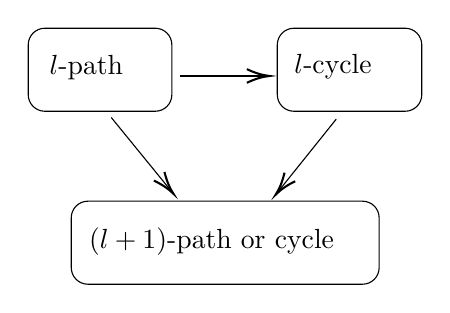
\begin{tikzpicture}[x=0.75pt,y=0.75pt,yscale=-1,xscale=1]
    % Rounded Rect [id:dp2247988663004169] 
    \draw   (100.6,84) .. controls (100.6,79.58) and (104.18,76) .. (108.6,76) -- (161.8,76) .. controls (166.22,76) and (169.8,79.58) .. (169.8,84) -- (169.8,108) .. controls (169.8,112.42) and (166.22,116) .. (161.8,116) -- (108.6,116) .. controls (104.18,116) and (100.6,112.42) .. (100.6,108) -- cycle ;
    % Rounded Rect [id:dp3322171879942837] 
    \draw   (220.6,84) .. controls (220.6,79.58) and (224.18,76) .. (228.6,76) -- (282.2,76) .. controls (286.62,76) and (290.2,79.58) .. (290.2,84) -- (290.2,108) .. controls (290.2,112.42) and (286.62,116) .. (282.2,116) -- (228.6,116) .. controls (224.18,116) and (220.6,112.42) .. (220.6,108) -- cycle ;
    % Rounded Rect [id:dp522325016929076] 
    \draw   (121.33,167.33) .. controls (121.33,162.92) and (124.92,159.33) .. (129.33,159.33) -- (261.67,159.33) .. controls (266.08,159.33) and (269.67,162.92) .. (269.67,167.33) -- (269.67,191.33) .. controls (269.67,195.75) and (266.08,199.33) .. (261.67,199.33) -- (129.33,199.33) .. controls (124.92,199.33) and (121.33,195.75) .. (121.33,191.33) -- cycle ;
    % Straight Lines [id:da4471732816066223] 
    \draw    (173.53,99) -- (214.87,99) ;
    \draw [shift={(216.87,99)}, rotate = 180] [color={rgb, 255:red, 0; green, 0; blue, 0 }  ][line width=0.75]    (10.93,-3.29) .. controls (6.95,-1.4) and (3.31,-0.3) .. (0,0) .. controls (3.31,0.3) and (6.95,1.4) .. (10.93,3.29)   ;
    % Straight Lines [id:da08077221270601986] 
    \draw    (140.6,119) -- (169.34,154.25) ;
    \draw [shift={(170.6,155.8)}, rotate = 230.81] [color={rgb, 255:red, 0; green, 0; blue, 0 }  ][line width=0.75]    (10.93,-3.29) .. controls (6.95,-1.4) and (3.31,-0.3) .. (0,0) .. controls (3.31,0.3) and (6.95,1.4) .. (10.93,3.29)   ;
    % Straight Lines [id:da17940502186011487] 
    \draw    (249,119.8) -- (221.05,154.64) ;
    \draw [shift={(219.8,156.2)}, rotate = 308.74] [color={rgb, 255:red, 0; green, 0; blue, 0 }  ][line width=0.75]    (10.93,-3.29) .. controls (6.95,-1.4) and (3.31,-0.3) .. (0,0) .. controls (3.31,0.3) and (6.95,1.4) .. (10.93,3.29)   ;

    % Text Nodes
    \draw (109.6,87.67) node [anchor=north west][inner sep=0.75pt]   [align=left] {$l$-path};
    \draw (227.6,87.27) node [anchor=north west][inner sep=0.75pt]   [align=left] {$l$-cycle};
    \draw (128.67,171) node [anchor=north west][inner sep=0.75pt]   [align=left] {$(l+1)$-path or cycle};
    \end{tikzpicture}
\end{center}

The algorithm considers two primary cases: when the object is a path and when it is a cycle.

\subsection{Path of Length $l$}

In this case, we start with a path \( P = \{x_1, e_1, \dots, x_{l}, e_{l}, x_{l + 1}\} \) of length \( l \). The goal is to find either a path of length \( l+1 \) or a cycle of length \( l \) or \( l+1 \). To assist in this process, we define the following variables:

\begin{itemize}
    \item \texttt{colors\_in\_path}: An array of size \( n \) where \texttt{colors\_in\_path[i]} is \texttt{True} if color \( i \) is used in the edges of the path.
    \item \texttt{vertices\_in\_path}: An array of size \( n \) where \texttt{vertices\_in\_path[i]} is \texttt{True} if vertex \( i \) is included in the path.
\end{itemize}

Let's divide the proof into two cases: when \( l \geq \left \lceil \frac{n}{2} \right \rceil \) and when \( l < \left \lceil \frac{n}{2} \right \rceil \).

\subsubsection{Case 1: \( l < \left \lceil \frac{n}{2} \right \rceil \)}

In this case, we select a color \( c \) that is not present among 
the edges of the current path. Since 
\( \deg(x_{l + 1}, c) \geq \left \lceil \frac{n}{2} \right \rceil \), 
and there are at most 
\( l < \left \lceil \frac{n}{2} \right \rceil \) 
vertices in the path, there must be a vertex 
\( y \) 
outside the path that is adjacent to 
\( x_{l + 1} \) via an edge in \( E(G_c) \). 
This guarantees that we can extend the path to a bigger path.

\begin{algorithm}[H]
    \caption{Path Extension for \( l < \left \lceil \frac{n}{2} \right \rceil \)}
    \begin{algorithmic}[1]
        \Function{Extend\_Path\_Small}{$G, P$}
        \State \textbf{assert} \( P.\text{size()} < \lceil \frac{n}{2} \rceil \)
        \State $last\_vertex \gets P.\text{back()}$
        \For{$color \in \{0, \dots, n-1\}$}
            \If{\textbf{not} $colors\_in\_path[color]$} \Comment{Search for an unused color}
                \For{$i \in \{0, \dots, n-1\}$}
                    \If{\textbf{not} $vertices\_in\_path[i]$} \Comment{Check vertices outside the path}
                        \State $edge \gets G.\text{check\_edge}(last\_vertex, i, color)$
                        \If{$edge \neq \text{None}$}
                            \State $vertices.\text{append}(i)$
                            \State $edges.\text{append}(edge)$
                            \State \Return Path($G$, $vertices$, $edges$) \Comment{Return extended path}
                        \EndIf
                    \EndIf
                \EndFor
            \EndIf
        \EndFor
        \State \textbf{assert False, "No valid extension found"}
    \EndFunction
    \end{algorithmic}
\end{algorithm}

The time complexity of this function is \( O(n) \). Since we 
only need to find a color that is not in the path’s colors 
,which takes \( O(n) \), and then locate a vertex outside 
the path that connects to the last vertex (also \( O(n) \)), 
the overall complexity remains linear in \( n \).

\subsubsection{Case 2: \( l \geq \left \lceil \frac{n}{2} \right \rceil \)}

First, remove the last edge and
vertex of the path and let $cx$ be a color that is not on the path and 
$cy$ be the color of the removed edge. We can check if the edge $\{x_1, x_{l}\}$ belongs to $G_{cx}$ or
to $G_{cy}$. If it does, we just found a cycle of size $l$. This can be done in $O(n)$ time complexity, the time need
to find a color outside the path and create the object Cycle. 


\begin{algorithm}[H]
    \caption{Part 1: Path Extension for \( l > \left \lceil \frac{n}{2} \right \rceil \)}
    \begin{algorithmic}
        \Function{Extend\_Path\_Big}{$G, P$}
            \State $cx \gets P.\text{edges}[-1].\text{color}$ \Comment{Color of the last edge in the path}
            \State $cy \gets \text{any color not in } colors\_in\_path$ \Comment{Find a color not in the path}
            \State $P.\text{pop\_back()}$ \Comment{Remove the last vertex from the path}
            \State $x \gets P.\text{vertices}[0]$ \Comment{First vertex in the path}
            \State $y \gets P.\text{vertices}[-1]$ \Comment{Last vertex in the updated path}

            \If{$edge \gets \text{check\_edge}(G, x, y, c) \neq \text{None}$}
                \State $vertices \gets P.\text{vertices.copy()}$
                \State $edges \gets P.\text{edges.copy()}$
                \State $edges.\text{append}(edge)$
                \State \Return Cycle($G$, $vertices$, $edges$) \Comment{Return cycle if found}
            \EndIf
        \EndFunction
    \end{algorithmic}
\end{algorithm}

We can now check if there exists a vertex $i$ outside the Path
such that $i$ is connects to the path on vertices $x_1$ and $x_l$
and uses colors $cx$ and $cy$, such as in the image below:

\begin{center}
    \tikzset{every picture/.style={line width=0.75pt}} %set default line width to 0.75pt        

    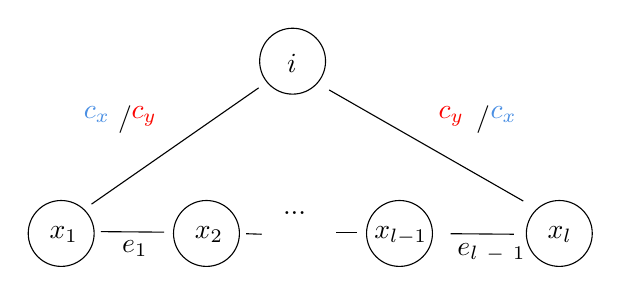
\begin{tikzpicture}[x=0.75pt,y=0.75pt,yscale=-1,xscale=1]
    %uncomment if require: \path (0,300); %set diagram left start at 0, and has height of 300
    
    %Shape: Circle [id:dp14076860311809425] 
    \draw  [color={rgb, 255:red, 0; green, 0; blue, 0 }  ,draw opacity=1 ] (100,135.88) .. controls (100,127.11) and (107.11,120) .. (115.88,120) .. controls (124.64,120) and (131.75,127.11) .. (131.75,135.88) .. controls (131.75,144.64) and (124.64,151.75) .. (115.88,151.75) .. controls (107.11,151.75) and (100,144.64) .. (100,135.88) -- cycle ;
    %Shape: Circle [id:dp9718918515389369] 
    \draw  [color={rgb, 255:red, 0; green, 0; blue, 0 }  ,draw opacity=1 ] (340,135.88) .. controls (340,127.11) and (347.11,120) .. (355.88,120) .. controls (364.64,120) and (371.75,127.11) .. (371.75,135.88) .. controls (371.75,144.64) and (364.64,151.75) .. (355.88,151.75) .. controls (347.11,151.75) and (340,144.64) .. (340,135.88) -- cycle ;
    %Shape: Circle [id:dp22152249244642985] 
    \draw  [color={rgb, 255:red, 0; green, 0; blue, 0 }  ,draw opacity=1 ] (170,135.88) .. controls (170,127.11) and (177.11,120) .. (185.88,120) .. controls (194.64,120) and (201.75,127.11) .. (201.75,135.88) .. controls (201.75,144.64) and (194.64,151.75) .. (185.88,151.75) .. controls (177.11,151.75) and (170,144.64) .. (170,135.88) -- cycle ;
    %Straight Lines [id:da5129055940889523] 
    \draw    (135,135) -- (165.5,135.25) ;
    %Straight Lines [id:da581278780757175] 
    \draw    (303.5,136) -- (334,136.25) ;
    %Shape: Circle [id:dp2164326053488742] 
    \draw  [color={rgb, 255:red, 0; green, 0; blue, 0 }  ,draw opacity=1 ] (263,135.88) .. controls (263,127.11) and (270.11,120) .. (278.88,120) .. controls (287.64,120) and (294.75,127.11) .. (294.75,135.88) .. controls (294.75,144.64) and (287.64,151.75) .. (278.88,151.75) .. controls (270.11,151.75) and (263,144.64) .. (263,135.88) -- cycle ;
    %Straight Lines [id:da9291156181154486] 
    \draw    (248.5,135.25) -- (258.5,135.25) ;
    %Straight Lines [id:da2577772310594443] 
    \draw    (205,136) -- (212.5,136.25) ;
    %Shape: Circle [id:dp2553341740528331] 
    \draw  [color={rgb, 255:red, 0; green, 0; blue, 0 }  ,draw opacity=1 ] (211.5,52.88) .. controls (211.5,44.11) and (218.61,37) .. (227.38,37) .. controls (236.14,37) and (243.25,44.11) .. (243.25,52.88) .. controls (243.25,61.64) and (236.14,68.75) .. (227.38,68.75) .. controls (218.61,68.75) and (211.5,61.64) .. (211.5,52.88) -- cycle ;
    %Straight Lines [id:da500585581947927] 
    \draw    (130.5,121.75) -- (211,65.75) ;
    %Straight Lines [id:da13872883018767035] 
    \draw    (338.5,120.25) -- (245,66.75) ;
    
    % Text Node
    \draw (109,131.4) node [anchor=north west][inner sep=0.75pt]    {$x_{1}$};
    % Text Node
    \draw (349,131.4) node [anchor=north west][inner sep=0.75pt]    {$x_{l}$};
    % Text Node
    \draw (179,131.4) node [anchor=north west][inner sep=0.75pt]    {$x_{2}$};
    % Text Node
    \draw (265.5,131.4) node [anchor=north west][inner sep=0.75pt]    {$x_{l-1}$};
    % Text Node
    \draw (221.5,124) node [anchor=north west][inner sep=0.75pt]   [align=left] {...};
    % Text Node
    \draw (144,137.9) node [anchor=north west][inner sep=0.75pt]    {$e_{1}$};
    % Text Node
    \draw (305.5,139.4) node [anchor=north west][inner sep=0.75pt]    {$e_{l\ -\ 1}$};
    % Text Node
    \draw (223.5,48.4) node [anchor=north west][inner sep=0.75pt]    {$i$};
    % Text Node
    \draw (125.5,73.4) node [anchor=north west][inner sep=0.75pt]    {$\textcolor[rgb]{0.29,0.56,0.89}{c_{x}}$};
    % Text Node
    \draw (321.5,73.4) node [anchor=north west][inner sep=0.75pt]    {$\textcolor[rgb]{0.29,0.56,0.89}{c}\textcolor[rgb]{0.29,0.56,0.89}{_{x}}$};
    % Text Node
    \draw (148.5,73.4) node [anchor=north west][inner sep=0.75pt]    {$\textcolor[rgb]{0.99,0.01,0.01}{c_{\textcolor[rgb]{0.98,0.03,0}{y}}}$};
    % Text Node
    \draw (142,73) node [anchor=north west][inner sep=0.75pt]   [align=left] {/};
    % Text Node
    \draw (296.5,73.4) node [anchor=north west][inner sep=0.75pt]    {$\textcolor[rgb]{0.99,0.01,0.01}{c}\textcolor[rgb]{0.99,0.01,0.01}{_{\textcolor[rgb]{0.98,0.03,0}{y}}}$};
    % Text Node
    \draw (314.5,73) node [anchor=north west][inner sep=0.75pt]   [align=left] {/};
    
    
    \end{tikzpicture}
    
\end{center}

This part can also be done on $O(n)$ time complexity with
the code below:

\begin{algorithm}[H]
    \caption{Part 3: Path Extension for \( l > \left \lceil \frac{n}{2} \right \rceil \)}
    \begin{algorithmic}
        \Function{Extend\_Path\_Big}{$G, P$}
            \For{$[c1, c2] \in [[cx, cy], [cy, cx]]$} \Comment{Try both color pairs}
                \For{$i \in \{0, \dots, n-1\}$}
                    \If{\textbf{not} $vertices\_in\_path[i]$} \Comment{Check vertices outside the path}
                        \State $edgeX \gets \text{check\_edge}(G, x, i, c1)$
                        \State $edgeY \gets \text{check\_edge}(G, y, i, c2)$
                        \If{$(edgeX \neq \text{None})$ and $(edgeY \neq \text{None})$}
                            \State $vertices \gets P.\text{vertices.copy()}$
                            \State $vertices.\text{append}(i)$
                            \State $edges \gets P.\text{edges.copy()}$
                            \State $edges.\text{append}(edgeY)$
                            \State $edges.\text{append}(edgeX)$
                            \State \Return Cycle($G$, $vertices$, $edges$) \Comment{Return cycle if found}
                        \EndIf
                    \EndIf
                \EndFor
            \EndFor

            \State \textbf{assert False, "No valid extension found"}
        \EndFunction
    \end{algorithmic}
\end{algorithm}

Let's define $I_1 = \{i \in [l - 2]: \{x_1, x_{i + 1}\} \in E_{G_cx}\}$ and 
$I_2 = \{i \in [2, l - 1]: \{x_i, x_{l}\} \in E_{G_cy}\}$. As 

Note that as we did not find a cycle yet, 

$$
|N_{G_cx}(x_1) \backslash V(P)| + |N_{G_cy}(x_l) \backslash V(P)| \leq n - l,
$$

otherwise, by Dirichlet Principle, we would have found a cycle
with the procedures above. Thus, we have that

$$
|I_1| + |I_2| \geq \frac{n}{2} + \frac{n}{2} - |N_{G_cx}(x_1) \backslash V(P)| - |N_{G_cy}(x_l) \backslash V(P)| \geq l.
$$

As we $I_1$ and $I_2$ share the same set of vertices of size
$l - 2$, $I_1 \cap I_2 \neq \emptyset$. Given an element
$i \in I_1 \cap I_2$, we can build a cycle with size $l$ with
the following crossing, removing edge $x_i$.

\begin{center}
\tikzset{every picture/.style={line width=0.75pt}} %set default line width to 0.75pt        

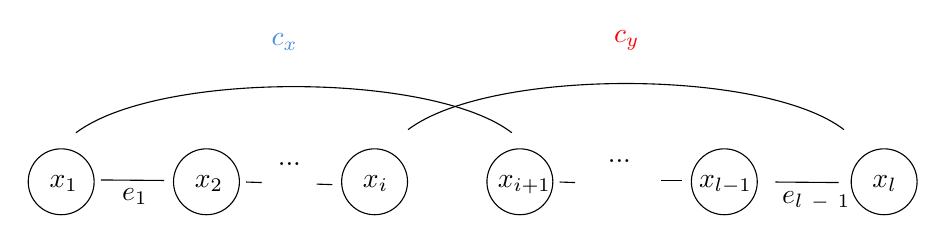
\begin{tikzpicture}[x=0.75pt,y=0.75pt,yscale=-1,xscale=1]
%uncomment if require: \path (0,300); %set diagram left start at 0, and has height of 300

%Shape: Circle [id:dp14076860311809425] 
\draw  [color={rgb, 255:red, 0; green, 0; blue, 0 }  ,draw opacity=1 ] (100,135.88) .. controls (100,127.11) and (107.11,120) .. (115.88,120) .. controls (124.64,120) and (131.75,127.11) .. (131.75,135.88) .. controls (131.75,144.64) and (124.64,151.75) .. (115.88,151.75) .. controls (107.11,151.75) and (100,144.64) .. (100,135.88) -- cycle ;
%Shape: Circle [id:dp9718918515389369] 
\draw  [color={rgb, 255:red, 0; green, 0; blue, 0 }  ,draw opacity=1 ] (496.5,135.88) .. controls (496.5,127.11) and (503.61,120) .. (512.38,120) .. controls (521.14,120) and (528.25,127.11) .. (528.25,135.88) .. controls (528.25,144.64) and (521.14,151.75) .. (512.38,151.75) .. controls (503.61,151.75) and (496.5,144.64) .. (496.5,135.88) -- cycle ;
%Shape: Circle [id:dp22152249244642985] 
\draw  [color={rgb, 255:red, 0; green, 0; blue, 0 }  ,draw opacity=1 ] (170,135.88) .. controls (170,127.11) and (177.11,120) .. (185.88,120) .. controls (194.64,120) and (201.75,127.11) .. (201.75,135.88) .. controls (201.75,144.64) and (194.64,151.75) .. (185.88,151.75) .. controls (177.11,151.75) and (170,144.64) .. (170,135.88) -- cycle ;
%Straight Lines [id:da5129055940889523] 
\draw    (135,135) -- (165.5,135.25) ;
%Straight Lines [id:da581278780757175] 
\draw    (460,136) -- (490.5,136.25) ;
%Shape: Circle [id:dp2164326053488742] 
\draw  [color={rgb, 255:red, 0; green, 0; blue, 0 }  ,draw opacity=1 ] (419.5,135.88) .. controls (419.5,127.11) and (426.61,120) .. (435.38,120) .. controls (444.14,120) and (451.25,127.11) .. (451.25,135.88) .. controls (451.25,144.64) and (444.14,151.75) .. (435.38,151.75) .. controls (426.61,151.75) and (419.5,144.64) .. (419.5,135.88) -- cycle ;
%Straight Lines [id:da9291156181154486] 
\draw    (405,135.25) -- (415,135.25) ;
%Straight Lines [id:da2577772310594443] 
\draw    (205,136) -- (212.5,136.25) ;
%Shape: Circle [id:dp8825188362565558] 
\draw  [color={rgb, 255:red, 0; green, 0; blue, 0 }  ,draw opacity=1 ] (251,135.88) .. controls (251,127.11) and (258.11,120) .. (266.88,120) .. controls (275.64,120) and (282.75,127.11) .. (282.75,135.88) .. controls (282.75,144.64) and (275.64,151.75) .. (266.88,151.75) .. controls (258.11,151.75) and (251,144.64) .. (251,135.88) -- cycle ;
%Shape: Circle [id:dp9134750344031234] 
\draw  [color={rgb, 255:red, 0; green, 0; blue, 0 }  ,draw opacity=1 ] (321,135.88) .. controls (321,127.11) and (328.11,120) .. (336.88,120) .. controls (345.64,120) and (352.75,127.11) .. (352.75,135.88) .. controls (352.75,144.64) and (345.64,151.75) .. (336.88,151.75) .. controls (328.11,151.75) and (321,144.64) .. (321,135.88) -- cycle ;
%Straight Lines [id:da6587077764610608] 
\draw    (356,136) -- (363.5,136.25) ;
%Straight Lines [id:da08873759090043654] 
\draw    (239,137) -- (246.5,137.25) ;
%Curve Lines [id:da934768158738368] 
\draw    (123,112.25) .. controls (163,82.25) and (295,83) .. (333,112.25) ;
%Curve Lines [id:da06750067448598662] 
\draw    (283,110.75) .. controls (323,80.75) and (455,81.5) .. (493,110.75) ;

% Text Node
\draw (109,131.4) node [anchor=north west][inner sep=0.75pt]    {$x_{1}$};
% Text Node
\draw (505.5,131.4) node [anchor=north west][inner sep=0.75pt]    {$x_{l}$};
% Text Node
\draw (179,131.4) node [anchor=north west][inner sep=0.75pt]    {$x_{2}$};
% Text Node
\draw (422,131.4) node [anchor=north west][inner sep=0.75pt]    {$x_{l-1}$};
% Text Node
\draw (378,124) node [anchor=north west][inner sep=0.75pt]   [align=left] {...};
% Text Node
\draw (144,137.9) node [anchor=north west][inner sep=0.75pt]    {$e_{1}$};
% Text Node
\draw (462,139.4) node [anchor=north west][inner sep=0.75pt]    {$e_{l\ -\ 1}$};
% Text Node
\draw (216,63.4) node [anchor=north west][inner sep=0.75pt]    {$\textcolor[rgb]{0.29,0.56,0.89}{c_{x}}$};
% Text Node
\draw (381,61.9) node [anchor=north west][inner sep=0.75pt]    {$\textcolor[rgb]{0.99,0.01,0.01}{c_{\textcolor[rgb]{0.98,0.03,0}{y}}}$};
% Text Node
\draw (219,125.5) node [anchor=north west][inner sep=0.75pt]   [align=left] {...};
% Text Node
\draw (260,131.4) node [anchor=north west][inner sep=0.75pt]    {$x_{i}$};
% Text Node
\draw (325,131.4) node [anchor=north west][inner sep=0.75pt]    {$x_{i+1}$};


\end{tikzpicture}

\end{center}

Then, for this case, we just need to find an intersection
for $I_1$ and $I_2$ and build the solution. This can also
be done in $O(n)$ with the code below:

\begin{algorithm}[H]
    \caption{Part 3: Path Extension for \( l > \left \lceil \frac{n}{2} \right \rceil \)}
    \begin{algorithmic}[1]
        \Function{Extend\_Path\_Big}{$G, P$}
            \For{$i \gets 1$ to $|P.\text{vertices}| - 2$}
                \State $u \gets P.\text{vertices}[i]$
                \State $v \gets P.\text{vertices}[i + 1]$
                \State $edgeX \gets \text{check\_edge}(G, x, v, cx)$
                \State $edgeY \gets G.\text{check\_edge}(G, u, y, cy)$

                \If{$(edgeX \neq \text{None})$ and $(edgeY \neq \text{None})$} 
                    \State $vertices \gets P.\text{vertices}[1:i] + [y] + \text{Reverse}(P.\text{vertices}[i + 1:l])$
                    \State $edges \gets P.\text{edges}[1:i - 1] + [edgeY]$

                    \For{$j \gets |P.\text{vertices}| - 1$ down to $i + 1$}
                        \State $vertices.\text{append}(P.\text{vertices}[j - 1])$
                        \State $edges.\text{append}(P.\text{edges}[j - 1])$
                    \EndFor
                    \State $edges.\text{append}(edgeX)$ \Comment{Add $edgeX$ to close the cycle}
                    \State \Return Cycle($G$, $vertices$, $edges$)
                \EndIf
            \EndFor
            \State \Return \text{None} \Comment{Return None if no cycle found}
        \EndFunction
    \end{algorithmic}
\end{algorithm}



\subsection{Cycle of length $n - 1 \neq \ell \geq \left \lfloor \frac{n}{2} \right \rfloor$}

\section{Cycle of length $n - 1$}




\pagestyle{mainmatter}
%!TeX root=../tese.tex

\chapter{Rainbow version of Ore's Theorem}
\label{chap:ore}

In 1960, Ore~(\cite{Ore_1960}) proved the following result.

\bigskip

 \ni {\textbf{Theorem 1 (Ore, 1960).}}
  \textsl{If $G = (V, E)$ is a simple graph of order  $n\geq 3$  such that 
  $d_G(u) + d_G(v) \geq n$ for all pair of non-adjacent vertices $u, v \in V$,
  then $G$ contains a Hamiltonian cycle.}

\bigskip
  
In what follows, we shall refer to the above sufficient condition as \emph{Ore's condition}. 
It is immediate that Ore's theorem generalizes Dirac's theorem. So, a natural question that arises
is whether an analogous  rainbow version of Ore's Theorem also holds. We conjecture that
the answer is yes. For the moment, we are able to prove that the following (weaker) result holds.

\bigskip

\ni{\textbf{Theorem 2.}}
\textsl{Let $n\geq 3$ and $G = G_0 \cup G_1 \cup \ldots \cup G_{n-1}$ be a
graph that is the union of $n$ pairwise edge-disjoint simple graphs
$G_i$ of order $n$, all defined on a same vertex set, each one
monochromatically edge colored but collectively using $n$ distinct
colors. If each $G_i$ satisfies Ore's condition, then $G$ has a
rainbow path and a rainbow cycle of length $n-1$.}

\medskip

\begin{proof} %Proof of Theorem 2

As in the proof of the rainbow version of Dirac's theorem, we consider two cases.

\begin{itemize}
  
\item[]\textbf{Case (a):} Given a rainbow path in $G$ of length $\ell < n-1$, how to extend it to a rainbow path
of length $\ell +1 $ or to a rainbow cycle of length $\ell$ ou $\ell + 1$. \\

\item[]\textbf{Case (b):} Given a rainbow cycle in $G$ of length $\ell < n-1$, how to obtain a rainbow cycle of length $\ell + 1$ or a rainbow path of length $\ell + 1$.

\end{itemize}

\smallskip

We note that, it is immediate that $G$ has a rainbow path of length~$2$. Thus, starting with such a path,
and considering the two cases above, we are able to construct a rainbow path in $G$ of length $n-1$
and a rainbow  cycle of length $n-1$. 

From now on, whenever we refer to a path or a cycle, these are always
rainbow, so we omit stating this (but it should be understood). To
simplify notation, as here we do not have many indices for the
vertices, when  referring to an edge with endpoints $u$ and $v$, instead of 
writing  $\{u,v\}$, we may represent it as $uv$.  Also, to state that
an edge $uv$ has color $c$, we write $uv \in G_c$.

\bigskip


\ni \textbf{Case (a):  Path of length $\ell$}


Let $P = (x_0, e_0, \dots, x_{\ell-1}, e_{\ell-1}, x_{\ell})$ be a
path in $G$ of length~$\ell$. \\

\smallskip

\begin{itemize}
  
\item[]\textbf{Case (a1): \(\ell < n/2 \)} \\


Let \( c \) be a color that is not in the path $P$, and let  \(u \coloneqq x_0\) and \(v \coloneqq x_{\ell}\). 
If \(uv \in G_c \), then by adding the edge $vu$ to $P$ we obtain a cycle of length \(\ell+1 \).
% 
Else, since \( uv \not\in G_c \), by Ore's condition, we have that
\( d_{G_c}(u) + d_{G_c}(v) \geq n \), and hence there is a
vertex \( w \notin V(P)\) such that \( uw \in G_c \) or
\( vw \in G_c \). Indeed, if such a vertex $w$ does not exist, then
\( d_{G_c}(u) \leq \ell \) and \( d_{G_c}(v) \leq \ell \). But
in this case, we have that 
\( d_{G_c}(u) + d_{G_c}(v) \leq 2\ell < n \), a contradiction.
Given such a vertex \(w\), we can construct a path of length \(\ell+1 \)
by appending $w$ to the path~$P$ and using precisely one of the edges \(uw\) or \(vw\).\\ 


\item[] \textbf{Case (a2): \( n/2 \leq \ell < n-1 \)} \\ 


Let $P'$ be the path obtained from $P$ after removing its last vertex~$x_\ell$, i.e., $P' = (x_0, e_0, \dots, x_{l-1})$. There are two colors, say $c_0$ and $c_1$, that are not present
in~$P'$. We may assume, without loss of generality, that
\(G_0 \coloneqq G_{c_0}\) and \(G_1 \coloneqq G_{c_1}\).

Let
\(u \coloneqq x_0\) and \( v \coloneqq x_{\ell-1}\). 
% 
For a vertex $w\in V(G_i)$, let \( d^{\text{out}}_{G_i}(w)\) denote
the number of neighbors of \(w\) in $G_i$ that are not in the path $P$
(they are out of $P$).  Analogously, let \(d^{\text{in}}_{G_i}(w) \)
denote the number of neighbors of \(w\) in $G_i$ that are in the path
$P$.
%
By definition, \( d^{\text{in}}_{G_i}(w) + d^{\text{out}}_{G_i}(w) = d_{G_i}(w) \).

If \(uv \in G_0 \) or \( uv \in G_1 \), then we can extend $P'$ to a cycle of length~\( \ell \)
by adding $uv$ to $P'$.  Else, by Ore's condition, \( d_{G_0}(u) + d_{G_0}(v) \geq n \) and \( d_{G_1}(u) + d_{G_1}(v) \geq n \).
If there exists a vertex \(w\) not in~$P'$ such that both \(uw \in G_0 \) and \(vw \in G_1 \), 
then we can extend $P'$ to a  cycle of length \( \ell + 1 \) by adding $w$ and the edges $vw$ and $wv$.
Such an extension is also possible if \( uw \in G_1 \) and \( vw \in G_0 \).


So, let us assume that such a vertex \(w\) does not exist. In this case, we have that 
\( d^{\text{out}}_{G_0}(u) + d^{\text{out}}_{G_1}(v) \leq n - \ell \) and
\( d^{\text{out}}_{G_1}(u) + d^{\text{out}}_{G_0}(v) \leq n - \ell \). 
So, we have that \( d^{\text{in}}_{G_0}(u) + d^{\text{in}}_{G_0}(v) + 
d^{\text{in}}_{G_1}(u) + d^{\text{in}}_{G_1}(v)  \geq 2 n - 2 ( n - \ell  ) = 2 \ell \). We must have that 
either \( d^{\text{in}}_{G_0}(u) + d^{\text{in}}_{G_1}(v) \geq \ell \) or 
\( d^{\text{in}}_{G_1}(u) + d^{\text{in}}_{G_0}(v) \geq \ell \).
Suppose, without loss of generality, that \( d^{\text{in}}_{G_0}(u) + d^{\text{in}}_{G_1}(v) \geq \ell \).
By the Pigeonhole Principle, there exists \(i\) such that
\( ux_i \in G_0 \) and \(vx_{i-1} \in G_1 \). Thus, we can construct a
a cycle of length \( \ell \).


\end{itemize}


\ni \textbf{Case (b):  Cycle of length $\ell < n - 1$}

Let \( C = \{x_0, e_0, \dots, x_{\ell-1}, e_{\ell-1}, x_{\ell}\} \) be a cycle
of length \(\ell < n - 1 \), and let  $c_0$ and $c_1$ be two colors that
are not present in~$C$.  Define \(G_0 \coloneqq G_{c_0}\) and \(G_1 \coloneqq G_{c_1} \).

\smallskip

\begin{itemize}
  
\item[]\textbf{Case (b1): \(\ell < n/2 \)} \\

As \(G_0\) satisfies Ore's condition, \(G_0\) is connected.  Then,
there exists an edge \( uv \in G_0 \) such that \( u \in C \)
and \( v \not\in C \).  Let \(w\) be a vertex adjacent to \(u\) in
\(C\).  If \(vw \in G_1\), then we have a rainbow cycle of
length \(\ell+1\).  Else, since \( vw \not\in G_1 \), by Ore's
condition, \( d_{G_1}(v) + d_{G_1}(w) \geq n \), and therefore there exists 
a vertex \( z  \not\in C\) such that \(vz \in G_1 \) or
\( wz \in G_1 \). Indeed, if not, we would have \( d_{G_1}(v) \leq \ell \)
and \( d_{G_1}(w) \leq \ell - 1 \), and we could conclude that 
\( d_{G_1}(v) + d_{G_1}(w) \leq 2\ell - 1 < n \), a contradiction.
%
Given such a vertex \(z\), we can construct a path of length \(\ell+1 \) if
\( vz \in G_1 \) or \( wz \in G_1 \). \\ 
% yw tirou  isso (como z nao pertence a z, z \neq w):  or we can construct a cycle of length \(\ell+1 \) if
% \( \{w, z\} \in G_1 \) and \(z \neq w\).

  
\item[]\textbf{Case (b2): \(n/2 \leq  \ell < n-1 \)}\\

Suppose there exists two vertices \( u, v \not\in C \) such that
\( uv \in G_0 \) and \( uv \not\in G_1 \).  By Ore's
condition, \( d_{G_1}(u) + d_{G_1}(v) \geq n \), which implies the
existence of a vertex \( w \in C \) such that \( uw \in G_1 \) or
\( vw \in G_1 \) --- otherwise
\( d_{G_1}(u) + d_{G_1}(v) \leq 2 (n - \ell - 1) < n \). Thus, we can
build a rainbow path of length \( \ell+1 \).  Otherwise, we have that for
all vertices \( u, v \not\in C \), 
\[ uv \in G_0 \Longleftrightarrow uv \in G_1. \]
Since \(G_0\) and \(G_1\) are connected graphs, if there is a pair of vertices 
\(u, v \not\in C\) such that \( uv \in G_0 \), then we can obtain a 
path with endpoint in \(u\) or \(v\) and in a vertex in the cycle,
that has  length at least \( \ell + 1 \).

We now assume that there is no pair of vertices \(u, v \not \in C\)
such that \( uv \in G_0 \).  Consider \( u, v \not\in C \). By Ore's
condition, \( d_{G_0}(u) + d_{G_0}(v) \geq n \) and
\( d_{G_1}(u) + d_{G_1}(v) \geq n \).  We also know that every
neighbor of \(u\) and \(v\) in \(G_0\) (resp. \(G_1\)) is in the
cycle~$C$, and therefore,
\( d_{G_0}(u) + d_{G_0}(v) + d_{G_1}(u) + d_{G_1}(v) \geq 2n > 2\ell \).
We can assume without loss of generality that
\( d_{G_0}(u) + d_{G_1}(v) > \ell \).  This means that there exist
adjacent vertices \(w\) and \(z\) in \(C\) such that \( uw \in G_0 \)
and \( zv \in G_1 \).  Thus, we can remove the edge $wz$ from $C$ and
add to the resulting path $C-wz$ the edges $uw$ and $zv$ and obtain a
path of length \(\ell+1\).

\end{itemize}

\end{proof}


\bigskip

We hope that from the rainbow Hamiltonian path in $G$ guaranteed to
exist by Theorem 2, we may succeed proving that $G$ has a
rainbow Hamiltonian cycle. This result would give us a theorem that is
precisely \emph{the rainbow version of Ore's theorem}. Anyway, we
think Theorem~2 is an interesting result by its own right.


\pagestyle{mainmatter}
%!TeX root=../tese.tex

\chapter{Conclusion}

The main objective of this work was to implement an efficient algorithm to find
the Rainbow version of Dirac's Theorem based on the work done by \cite{Joos_2020}.
The biggest challenge found in the implementation done in \autoref{chap:algorithmic} was 
finding a $\mathcal{G}$-transversal of length $n$ from a $\mathcal{G}$-transversal of length $n - 1$.

A battery of tests was also made to test our implementation.

We study the Rainbow version of Ore's Theorem, which is a generalization of
the Rainbow version of Dirac's Theorem. Although we do a proof similar
to \cite{Joos_2020} to prove the can find a 
$ \mathcal{G} $-transversal that is a cycle of length $ n - 1 $, it remains
to be seen if there is a proof of existence of a 
$ \mathcal{G} $-transversal that is a Hamiltonian cycle.

%%%%%%%%%%%%%%%%%%%%%%%%%%%% APÊNDICES E ANEXOS %%%%%%%%%%%%%%%%%%%%%%%%%%%%%%%%

%%%%%%%%%%%%%%% SEÇÕES FINAIS (BIBLIOGRAFIA E ÍNDICE REMISSIVO) %%%%%%%%%%%%%%%%

\backmatter
\pagestyle{backmatter}
\addtocontents{toc}{\vspace{2\baselineskip plus .5\baselineskip minus .5\baselineskip}}
\printbibliography[
  title=\refname\label{sec:bib}, % "Referências", recomendado pela ABNT
  title=\bibname\label{sec:bib}, % "Bibliografia"
  heading=bibintoc, % Inclui a bibliografia no sumário
]

\end{document}
